\section{Experimental Results and Analysis}
We first conduct Logistic Regression of several features scene specifically, then analyze the prominent factors behind to understand the relationship between the voice of dogs and humans.

\subsection{Results of Distinctiveness of Dog's Home Country}
\label{sec:main}


% \KZ{Make the fonts in the graph at least twice as big}
% \KZ{Don't use the word ``discrepancy''. It has a different meaning.}
% \KZ{Never mention fusion experiment before} The fusion experiment shows that the barks of Shiba Inu dogs are influenced by the scene context.

\begin{table}[th]
    \setlength\tabcolsep{3.5pt}
	\scriptsize
	\centering
	\begin{tabular}{l|llllllll}
		\toprule
		\multicolumn{1}{c|}{acc(\%)}        & play   & alone & eat   & fight & run   & walk & stranger & bath  \\
		\midrule
		\multicolumn{1}{c|}{play}           & -      & 74.05 & 72.99 & 67.55 & 74.50 & 70.57 & 70.25 & 72.39    \\
		\midrule
		\multicolumn{1}{c|}{alone}          & \textbf{74.05}  & -     & 71.35 & 71.93 & 71.79 & 67.12 & 67.50 & 70.65    \\
		\midrule
		\multicolumn{1}{c|}{eat}            & 72.99  & 71.35 & -     & 73.91 & 69.31 & 67.98 & 70.67 & 68.06    \\
		\midrule
		\multicolumn{1}{c|}{fight}          & 67.55  & 71.93 & 73.91 &  -    & 72.06 & 69.48 & 69.52 & 69.54  \\
		\midrule
		\multicolumn{1}{c|}{run}            & 74.50  & 71.79 & 69.31 & 72.06 & -     & 50.02 & 67.72 & 71.62    \\
		\midrule
		\multicolumn{1}{c|}{walk}           & 70.57  & 67.12 & 67.98 & 69.48 & \textbf{50.02} & -     & 64.18 & 69.34\\
		\midrule
		\multicolumn{1}{c|}{stranger}       & 70.25  & 67.50 & 70.67 & 69.52 & 67.72 & 64.18 & -     & 69.98\\
		\midrule
		\multicolumn{1}{c|}{bath}           & 72.39  & 70.65 & 68.06 & 69.54 & 71.62 & 69.34 & 69.98 & -  \\
		\bottomrule
	\end{tabular}
	\caption{We conduct Logistic Regression on filterbank features to distinguish barks of one scene from another scene. Then we get the scene classification accuracy.}
	\label{table:fusion}
\end{table}

We conduct the confusion experiment, which tends to distinguish barks of one scene from those of another scene, and find that scene information has influence on the voice of dogs. Thus we conduct classification generally with all the scenes mixed up and individually with only one scene per time in \figref{fig:acc}. From the confusion experiment in \tabref{table:fusion}, most of the scene contexts will have an specific influence on the voice of dogs compared to other scenes. Except for the scene walk and run, which the model could not classify. Scene ``alone'' and scene ``play'' are the most different pair.

\begin{figure}[th]
	\centering
	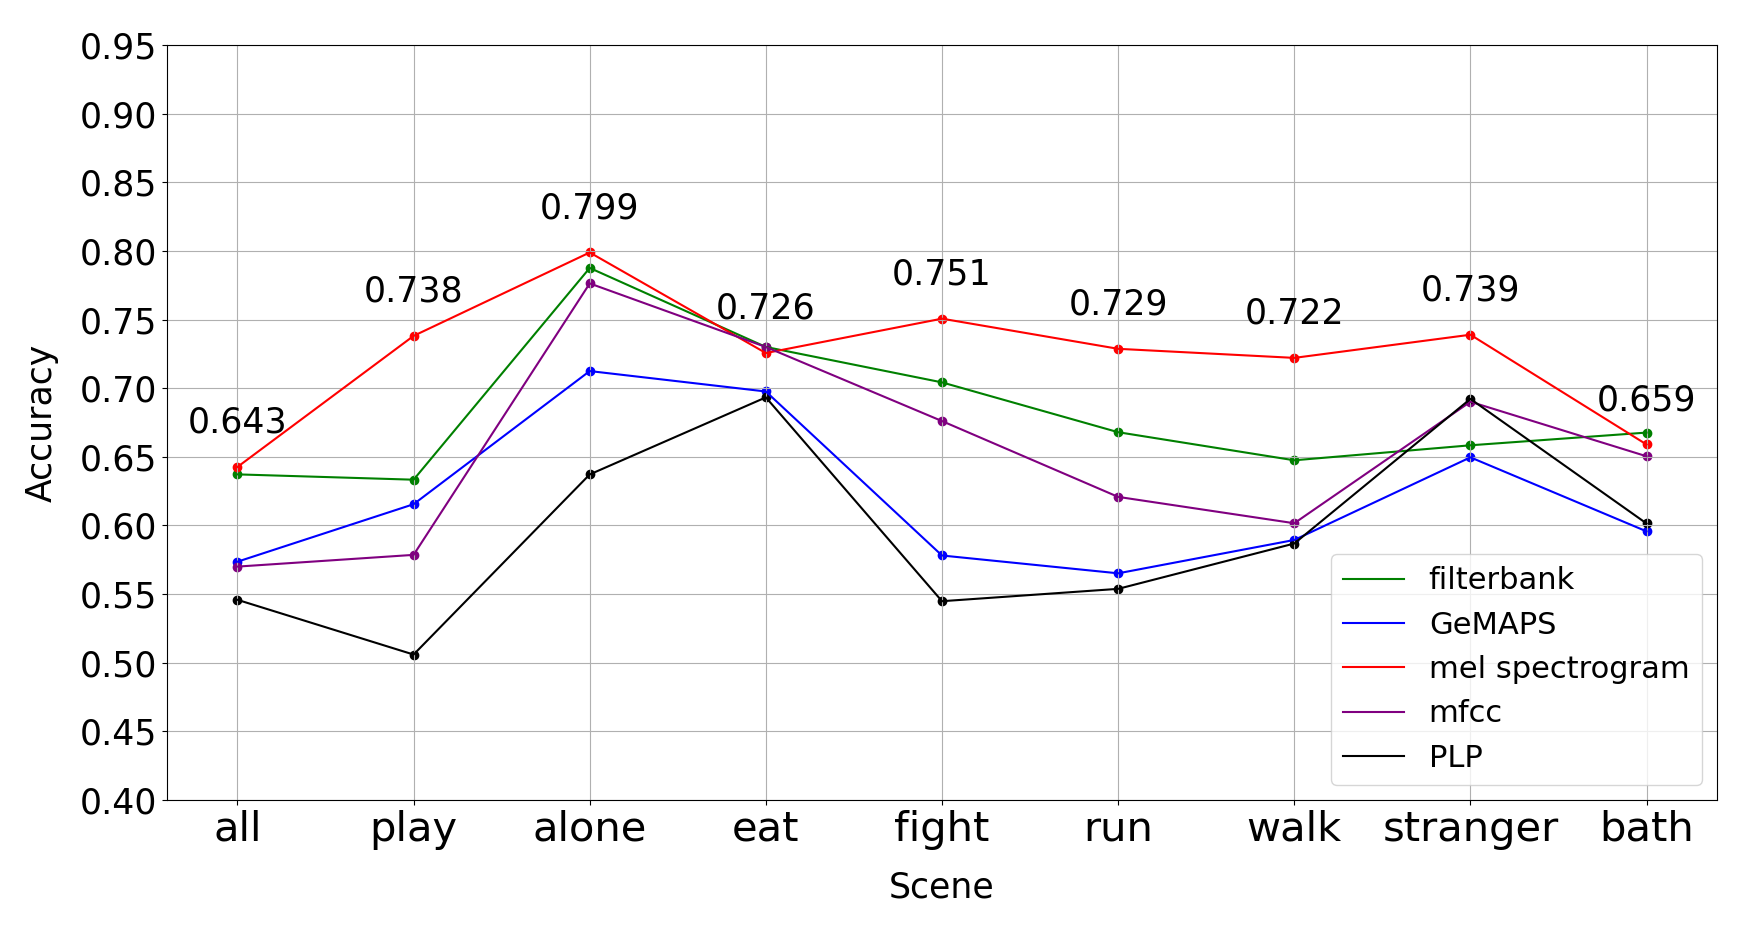
\includegraphics[width=\columnwidth]{acc.png}
	\caption{We conduct the classification experiment to distinguish Japanese dogs from English dogs. The classification accuracy of Logistic Regression on five features are showed above. The mel spectrogram performs best, with other features all being discriminative. We label the accuracy of the mel spectrogram.}
	\label{fig:acc}
\end{figure}


The five audio features that we use share the same tendency for different scenes though show different performances. We find that in scene-specific classification, the accuracy is higher than that in general classification with scenes mixed up, which is due to the noise of scene-specific information.

The best feature mel spectrogram displays an average accuracy of 73.27\% among scene-specific experiments, which reveals the difference caused by the language environments.



\subsection{Results of Prominent Factors}
\label{sec:prominentfactor}
We select five final prominent factors  as shown in bold \tabref{table:prominentfactor} according to the selection routine.
%\KZ{Where are the results?}

\begin{table}[th]
	\centering
	\scriptsize
	\begin{tabular}{l|ll}
		\toprule
		    Dimension & Coef  & Overlap    \\
		\midrule
	    \textbf{StddevUnvoicedSegmentLength} & \ 0.5956  & 7(/8)   \\
		\textbf{StddevVoicedSegmentLengthSec} & \ 0.4316   & 6(/8)\\
		F1bandwidth\_sma3nz\_stddevNorm & \ 0.4164 & 3(/8)  \\
		\textbf{MeanVoicedSegmentLengthSec} & \ 0.3128 & 5(/8)\\
		loudness\_sma3\_percentile50.0 &\ 0.3107 & 3(/8)\\
		F0semitoneFrom27.5Hz\_sma3nz\_stddevNorm & \ 0.2144 & 4(/8)\\
		\textbf{loudness\_sma3\_stddevNorm} & -0.2137 & 6(/8)\\
		\textbf{slopeUV0-500\_sma3nz\_amean} & -0.6541 & 5(/8)\\
		\bottomrule
	\end{tabular}
	\caption{Alternative coefficients and selection. All the dimensions~\cite{eyben2015geneva} consist of $D$. The bold dimensions are those selected as prominent factors.}
	\label{table:prominentfactor}
	 %\KZ{Give a cite for these long and complex feature names.}
\end{table}

The five final prominent factors above(in bold font)  could be divided into three kinds by their physical meaning. The first three are related to segment length, the fourth one is related to loudness and the last one is related to frequency. All the dimensions including the five above in GeMAPS are high-level statistics functions(HSFs) based on low-level descriptors(LLDs).


\textbf{The StddevUnvoicedSegmentLength} means the standard deviation of unvoiced segments length. This feature captures the pause length in speech signal, which leads to the difference in articulation rate. \textbf{The StddevVoicedSegmentLengthSec} means the standard deviation of the continuous voiced regions length per second, which can also be interpreted as the pseudo syllable rate. It has to do with the speed of speech and the density of syllables in a word. \textbf{The MeanVoicedSegmentLengthSec} means the average length of the continuous voiced regions per second.

% 前三个时间相关维度 总结
As for the 3 factors introduced above, they describe the temporal features of the voice. And the coefficient of these factors are all above zero, which may reveal that compared to that in Japanese environment, barks in English environment of dogs are likely to have more unvoiced segments in a sentence, and for each word, it may takes a longer time. This is consistent with the recognition of human langrage that Japanese is a so called "Syllable-timed" language with a more regular pattern of syllabic duration and fewer syllables per word\cite{arai1997temporal, greenberg1997origins}.

%loudness
\textbf{The loudness\_sma3\_stddevNorm} is the estimation of sound intensity, here is the mean loudness. We'll only take it as the audio sampling difference while recording.

%slopeUV
\textbf{The slopeUV0-500\_sma3nz\_amean} is the mean spectral slope 0-500Hz of unvoiced regions. Considering that the coefficient is under zero, and we take $y$ as 1 when the language environment belongs to English, the data shows that dogs from a Japanese language environment are more likely to generate 0-500Hz voice, which is low-frequency. Related to human language, the low-frequency band is more essential to Japanese\cite{ueda2010effects,lo18soundfreq}. What we find in dog language is consistent with this rule.

% What we find abo
% General understanding is that the frequency of English is higher than that of Japanese~\cite{ueda2017acoustic}, which is consistent with our experimental results here.
% 似乎和上一段重复了

\begin{figure}[H]
	\centering
	\subfigure[Barks under English Env.]{
	    \label{Fig.suben}
		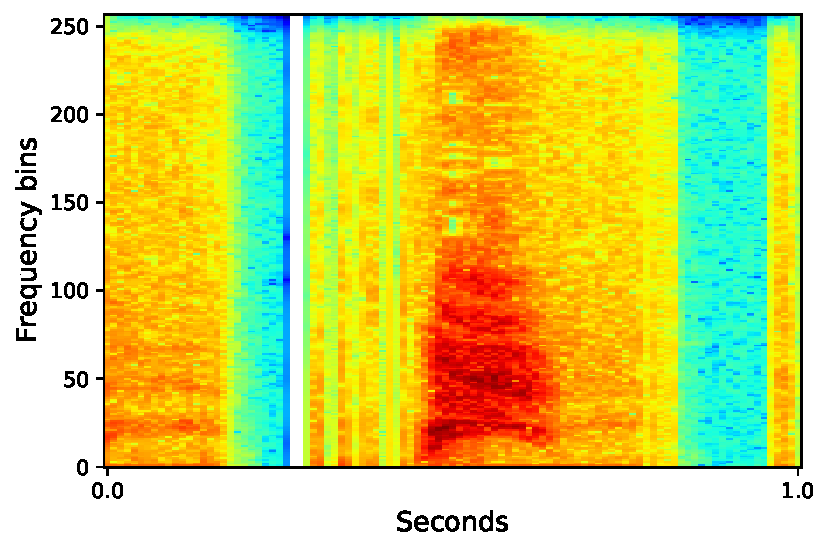
\includegraphics[width=0.48\linewidth]{dog_spec_en.pdf}}
	\subfigure[Barks under Japanese Env.]{
		\label{Fig.subja}
		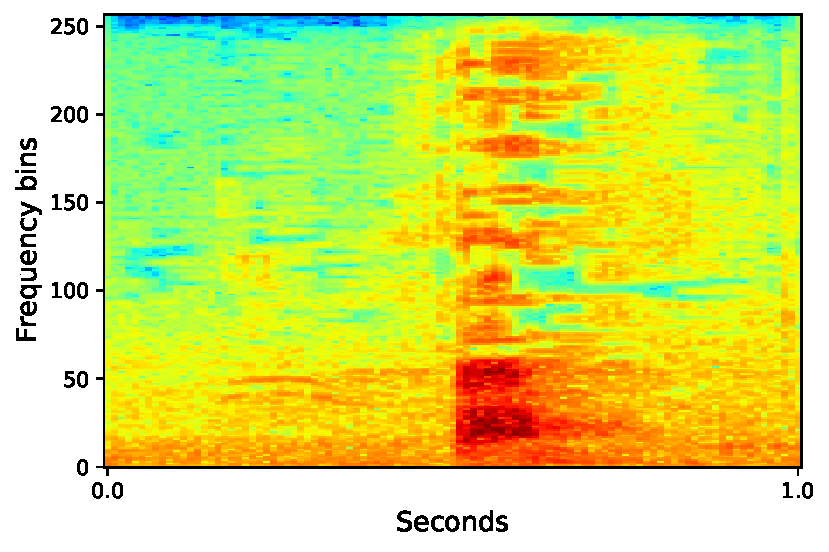
\includegraphics[width=0.48\linewidth]{dog_spec_ja.pdf}}
	\caption{The spectrogram of two audio samples which are from different language environments. They share the same scene Fight.}
	\label{Fig.sample}
\end{figure}

Here we list two typical samples from two language environments~\figref{Fig.sample}. It is clear that barks under English environment contain more unvoiced segments(the blue part) while the frequency of those barks under Japanese environment is closer to the low frequency region.






















